\documentclass[12pt]{article}

\usepackage{url} % websites in bib
\usepackage{hyperref}
\usepackage[a4paper,left=1in,right=1in,top=1in,bottom=1in]{geometry} % margins
\usepackage{paralist} % compact enumerates

\usepackage{graphicx}
\usepackage{caption}
\usepackage{subcaption}

\usepackage{amsmath}

\usepackage{multirow}

\usepackage{float} % figure placement

% Keywords command
\providecommand{\keywords}[1]
{
	\small	
	\textbf{\textit{Keywords---}} #1
}

\begin{document}
	\title{Clustering beer text reviews using the K-means algorithm}
	\author{Stefan Sebastian, 242}
	\date{}
	\maketitle
	
	\begin{abstract}
	Beer is the most popular alcoholic drink and has been around for a long time. In addition, a craft beer revolution is going on at the moment with a lot of new varieties coming out and being actively discussed by enthusiasts. Beer marketers could profit if they had an automated way of processing the thousands of reviews published on beer dedicated websites. This paper presents such a solution of extracting information from beer review data by unsupervised learning. A dataset of around 85 thousand reviews is analyzed by extracting Tf-Idf information from each row and then passing that into a K-means clustering algorithm. The resulting clusters are then associated with the most common beer style of the elements inside. This allows us to measure the correlation between reviews and the type of beer being reviewed. A discussion is then made based on the terms with the largest weights for each cluster center. The model obtains a F1 score of 0.53 on a 9 label classification problem indicating that there is indeed a correlation between a beer's review and its style.
	\end{abstract}

	\keywords{beer reviews, clustering, natural language processing}

	\newpage
	\tableofcontents
	\newpage
	
	\section{Introduction}
	\subsection{Motivation}
	Beer is one of the oldest and most popular alcoholic drinks. It is a staple drink in many societies and has been around ever since the formation of human civilizations, with evidence that dates it to more than 10,000 years ago\cite{BeerArticleTime}. It's popularity is attributed to having a moderate quantity of alcohol, which leads to more positive drinking experiences, and the fact that it can be drunk at any social event\cite{BeerArticleTime}.
	
	The global beer market was valued at 593\$ billion and is expected to rise to 685\$ billion by 2025\cite{BeerStats}. The most popular beer style is by far lager, but others are rising in popularity. Craft beer is a type of beer that is produced in microbreweries, in a traditional style and with an emphasis on taste and variety. The global craft beer market accounted for 38\$ billion and is growing at an explosive rate of 14.1\% each year\cite{CraftBeerStats}.
	
	\subsection{The tackled problem}
	It is obvious that there is a huge public interest in this drink, and any insights into what consumers think about beer could have serious economic benefits. This paper presents an experiment on extracting information using unsupervised learning on beer reviews, specifically through clustering methods. The algorithm works on a dataset consisting of textual descriptions of various beers, alongside a label indicating the type of beer which is described, which were made by beer enthusiasts all over the world, through the BeerAdvocate website. 
	
	The main goals are to find natural clusters among beer descriptions and to determine what words are used to describe similar beers. Also, the clusters are analyzed by the most common beer styles to see if there is a correlation between reviews and beer types.
	
	\subsection{Paper outline}
	The introductory section contains the motivation for the experiment and some insights into the studied domain. A short list of objectives is also put forth. The second section is a short survey of related work in terms of text clustering, review analysis and beer data mining. Next, the dataset used for the experiment is presented along with the exploratory data analysis and preprocessing techniques.
	
	The solution description section starts with a detailed presentation of the proposed model for data analysis. This is followed by some implementation discussion in subsection 'Technologies used'. Finally, the reasoning behind the selection of parameters for the model is given.
	
	The evaluation section describes the metrics and methodologies used to measure the performance of the proposed model. A concrete set of results is presented which is followed by some discussion based on the shape and means of the discovered clusters. Finally, the conclusion reiterate the results and propose some plans for future research.
	
	\section{Related work}
	
	\subsection{Text clustering}
	A comprehensive review on text document clustering similarity measures was published by Anna Huang\cite{TextClustering}. The paper describes a complete text clustering process with emphasis on distance measurements. Features are extracted using the tf-idf method and the clustering algorithm is the basic K-means variant. A set of similarity measures are studies such as cosine similarity, euclidean distance, Jaccard coefficient, etc. The datasets considered vary from news to scientific articles.
	
	An implementation of a Scatter-Gather document browsing system was presented by Larsen and Aone\cite{ScatterGather}. The system applies document clustering on the whole dataset, then when the user selects a group, it clusters the selected group into smaller groups. This operation can be extends until each group contains only one document. The algorithm used by the system is K-means with an improvement in seed selection consisting in updating the initial means after every point assignment. The algorithm uses as a feature extraction method the tf-idf vectorizer.
	
	An interesting approach to text clustering is the one developed by Hu et al.\cite{WikipediaKmeans}. Their method consists of enriching text information by using Wikipedia concept and category data. A dataset was made from Wikipedia articles related to different concepts. When a document is evaluated the term weight is calculated using the combined tf-idf score from the training and the Wikipedia concept dataset. The category score is built by analyzing the most important concepts of the document. The clustering algorithm used in the experiment was spherical K-means. This method was tested on three datasets and was shown to obtain better results than simple clustering over tf-idf scores.
	
	\subsection{Review analysis}
	Most papers on review analysis are focused on extracting information about aspects present in the review. For example, Lu et al.\cite{LARA} propose an algorithm for inferring the aspects considered in a review and assigning a score to them, and use it on hotel reviews from tripadvisor. The algorithm, called LARA, works in two steps. In the first step, given some keywords for the aspects, it associates each sentence in a review with the aspect for which it has the biggest overlap. In the second step, it computes a score for each aspect based on the sentiments present in the sentences found in previous steps.
	
	Another direction of review analysis is to use linguistic rules in a constrained domain. For instance, Iacob and Rachel\cite{MARA}, created an algorithm for automatically extracting and scoring feature request from mobile application reviews. The algorithm uses a set of 237 rules which were build by manual analysis of review data. An example rule is "(adding) \textless request\textgreater would (\textless ADVERB\textgreater) be \textless POSITIVE-ADJECTIVE\textgreater". The Latent Dirichlet Allocation algorithm is then used on the discovered feature requests in order to find topics.
	
	\subsection{Experiments on beer datasets}
	McAuley and Leskovec\cite{ExperienceReview} built a recommender system that adapts to user experience. The motivation was that the users' preferences evolve as they acquire experience. The datasets used for the experiment included the BeerAdvocate review dataset\cite{BeerAdvocateData} because of the fact that beer is one of the most widespread acquired tastes. The experience label is learned by the model by using rating and timestamp data.
	
	Braun and Timpe\cite{BeerWineReviews} scrape data from BeerAdvocate, RateBeer and CellarTracker websites. These contain user text reviews and numerical ratings for different types of beer and wine. The goal of the experiment is to predict scores based on the given review. The features are extracted using the bag-of-words model for single words an bigrams. To obtain more relevant features, the input data is stemmed, cleared of stop words, and the tokens are tagged by part of speech and only adjectives, nouns, verbs and adverbs are kept. The algorithms used for classification are Naive Bayes and Support Vector Machines. The model obtained an accuracy of up to 87\%.
	
	\section{Dataset}
	The dataset used for this experiment is a collection of beer reviews taken from the BeerAdvocate website. The original dataset was made up out of 1.5 million user reviews, from 33387 different users, collected between 1998 and 2011. It is not available at this time but I found a subset of around 500 thousand reviews on data.world\cite{BeerAdvocateData}. 
	
	The data is in csv format, each row containing various information like: beer name, beer style, alcohol content, scores for taste, appearance, aroma and a textual review. The only columns considered for this experiment were the beer style and the text review.
	
	On exploratory data analysis, 407 duplicate and 119 missing reviews were found. Also there are 104 distinct beer styles and the amount of data for each of them is quite imbalanced as can be see in figure \ref{fig:initialDistribution}, where each bar represents a beer style with a size proportional to the number of reviews for it.
	
	\begin{figure}[h]
		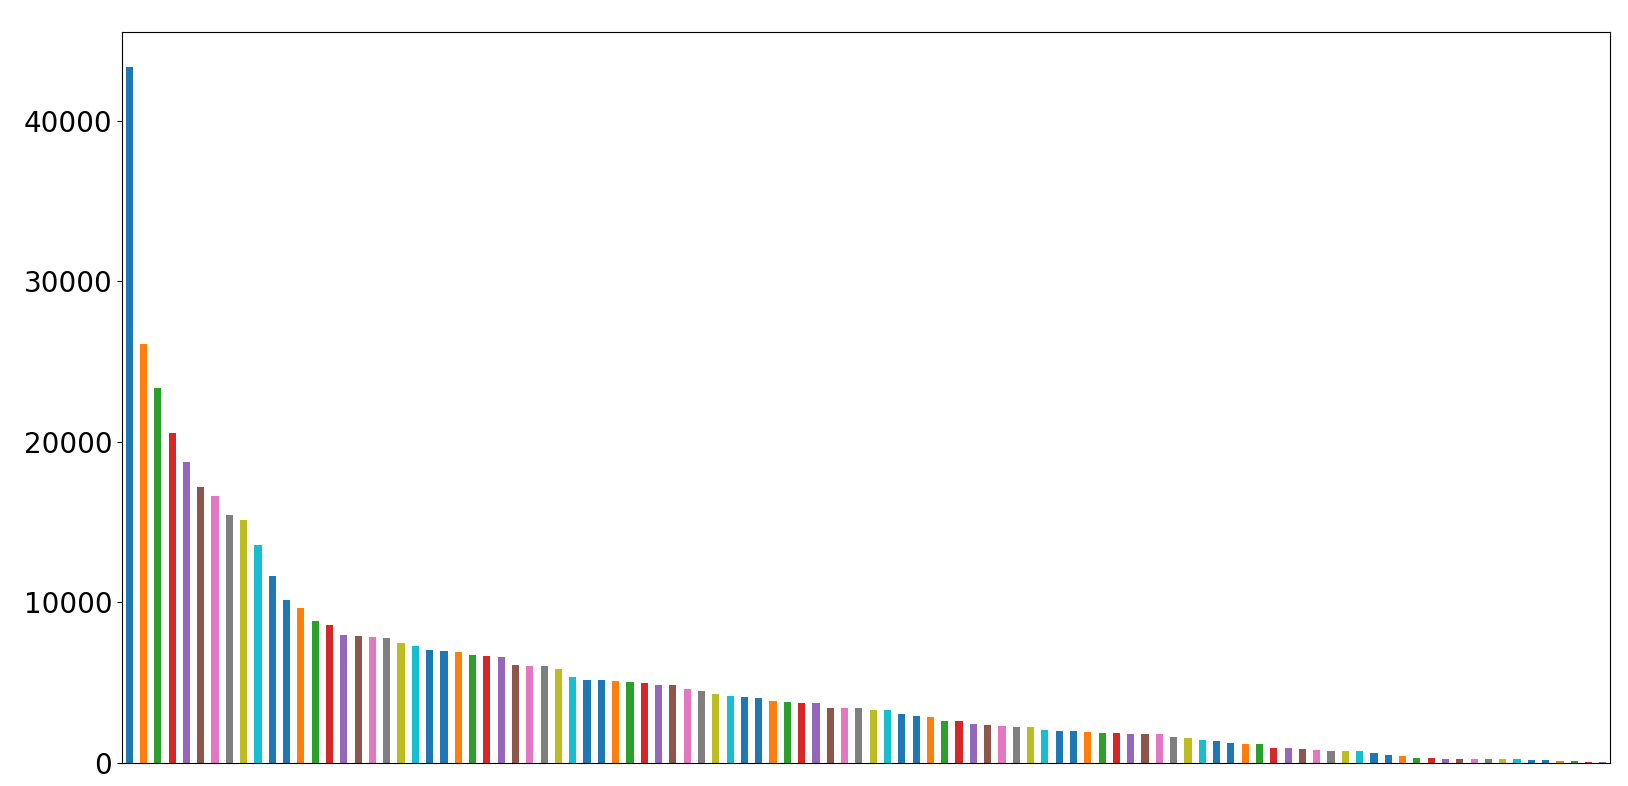
\includegraphics[width=\linewidth]{resources/InitialDistribution.png}
		\caption{A plot of the number of reviews per beer style}
		\label{fig:initialDistribution}
	\end{figure}

	The first step in preprocessing this dataset was to remove rows containing duplicates and missing values in the columns that are relevant for the experiment: beer style, text review. Next, some of the styles for which there wasn't a lot of data available were dropped, as they would be outliers for clustering. The threshold for this cut was chosen arbitrarily at 7000 reviews. 
	
	Upon inspection of the beer styles present in the dataset, a fine granularity was observed. For example, the difference between American Pale Ale and American India Pale Ale is minimal and not very rigorous. This and other similar cases would only confuse the classifier. For this reason, a mapping was made for each style to a broader category, using the taxonomy published by BusinessInsider\cite{BeerTaxonomy}. 
	
	The final mapping can be seen in figure \ref{fig:styleMapping}. Finally, a balanced dataset is built by selecting the minimum value for which we have an equal distribution of reviews per beer style, which is around 9500 per style. The analyzed dataset is made through random sampling of 9500 values for each of the remaining beer styles.
	
	\begin{figure}
		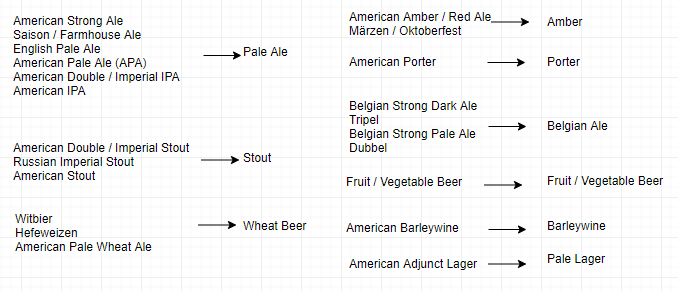
\includegraphics[width=\linewidth]{resources/MappingDiagram.png}
		\caption{Mapping of beer styles from the original dataset}
		\label{fig:styleMapping}
	\end{figure}

	\section{Solution description}
	\subsection{Model overview}
	In brief, the model proposed by this paper for solving the problem of extracting information from beer text reviews is made up out of two parts. Firstly, numerical features are extracted for each review using the Tf-Idf vectorizer, after applying some natural language processing techniques such as: stop word removal, tokenizing, stemming. The second step is to find natural clusters using the data points extracted previously. A classic clustering algorithm is used, K-means, with two different seed selection methods: random seeds and k-d trees. The resulting clusters are then evaluated based on initial beer style labels and the dominant terms in each cluster. 
	
	A more detailed descriptions of the methods used in the model is given in the next section, which aims to give the reader a theoretical background for understanding the proposed solution.

	\begin{figure}[H]
		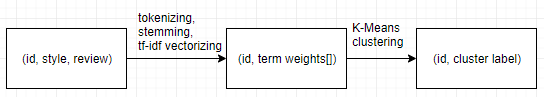
\includegraphics[width=\linewidth]{resources/model.png}
		\caption{Diagram of the transformations on the dataset}
		\label{fig:modelOverview}
	\end{figure}

	\subsection{Theoretical background}
	
	\subsubsection{Natural language processing}
	Natural language processing is a field in Computer Science which deals with extracting information from unmodified human language. Many artificial intelligence applications use datasets containing natural language text, however most algorithms are not designed to process this kind of data. Consequently, there are techniques for extracting numerical features from sentences, such as the Tf-Idf vectorizer. 
	
	Tf-Idf\cite{TfIdfBook} stands for term frequency-inverse document frequency and is the most popular method for weighting terms in a document. In brief, the importance of a word is proportional to the number of times it appears in a document and inversely proportional to the number of documents it appears in. Therefore, each document (a beer review, for the current experiment) will have a number of features equal to the number of considered words with a value indicating how relevant that word is for the document. The considered words can be all words from the combination of all documents in the initial dataset however that could be a huge number so a limit is usually chosen by the programmer.
	
	Before applying a technique such as Tf-Idf there needs to be a clear separation of words in the document. Here, the tokenizing process is applied. Tokenizing means splitting the document into words by applying some rules, usually by white spaces. Stop words, are terms which appear a lot in natural language but which do not provide meaningful information, such as: a, the, that, and are consequently removed before tokenizing. Another notable process is stemming, which reduces a word to its root form, for example the words: fishy, fishing, fished, will all become fish. This is useful because it allows the algorithm to group words which refer to the same concept. The algorithm selected for this experiment is the Snowball Stemmer\cite{SnowballStemmer}, which works by defining a set of rules for replacing word endings.

	\subsubsection{Clustering}
	Clustering is a field of data analysis whose purpose is to organize points, or objects into natural clusters. In other words given N objects described by a set of features, find a number of groups, such that objects in the same cluster are similar to each other and different from objects in other clusters\cite{DataClustering50yearsBeyondKmeans}. Given that there is no rigorous definition of similarity and that clusters in real data can overlap there are multiple algorithms and difference measures proposed in research.
	
	\paragraph{K-means}
	The K-means algorithm was discovered independently in multiple scientific fields around the same time and its name comes from a paper published by MacQueen in 1967\cite{DataClustering50yearsBeyondKmeans}. Despite being so old, this method is still widely used in clustering tasks because of its efficiency, simplicity and proven success. This was asserted by professor Anil K. Jain, who is an expert in the field of clustering, and believes K-means will remain a very popular algorithm in the future.
	
	The main goal of this algorithm is to minimize the distance between cluster centers and points assigned to them, which is a NP-hard problem. For this reason K-means is a greedy algorithm and has a chance to get stuck in local minimum instead of the best solution\cite{DataClustering50yearsBeyondKmeans}.
	
	A basic version of the K-means algorithm is\cite{AlgorithmsForClusteringData}:
	\begin{compactenum}
		\item Select an initial partition with K clusters and repeat 2 and 3 until the point membership no longer changes
		\item Assign each point to the closest center
		\item Update cluster centers based on the new assignment
	\end{compactenum}

	The most common seed selection method is to choose k random points, and then, to avoid scenarios in which this choice falls upon outliers or local optima, to repeat the K-means algorithm for a number of times. However, there are more efficient initialization methods, such as the k-d trees method.
	
	\paragraph{K-d trees}
	\begin{figure}[h]
		\centering
		\begin{subfigure}{.5\textwidth}
			\centering
			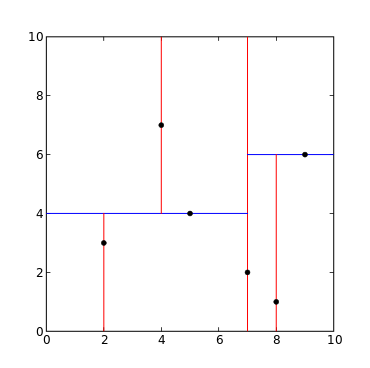
\includegraphics[width=.9\linewidth]{resources/Kdtree_2d.png}
			\caption{An example of a 2d k-d tree\cite{KdTreeFig1}}
		\end{subfigure}%
		\begin{subfigure}{.5\textwidth}
			\centering
			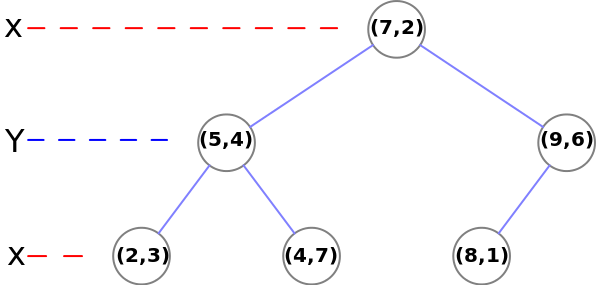
\includegraphics[width=.9\linewidth]{resources/Tree_0001.png}
			\caption{The data structure\cite{KdTreeFig2}}
		\end{subfigure}
		\caption{K-d tree graphic representation}
		\label{fig:kdtree}
	\end{figure}
	
	A k-d tree, introduced by Jon L. Bentley\cite{KdTree}, meaning k-dimensional tree is a data structure used to organize points in k-dimensional space, which is useful for partitioning data and optimizing multidimensional queries. The algorithm for building such a tree is recursive: select a point in the current dataset, choose a dimension, create a node of the selected point with a left subtree made out of the points with a lower value on the chosen dimension and a right subtree with the others. The space complexity for this structure is O(n) and all operations have an average time complexity of O(log n) and O(n) in the worst case. 
	
	An implementation of seed selection based on the k-d structure is proposed by Redmond and Heneghan\cite{KdTreeKmeans}. The reason for using this data structure is to gain information about the density of the dataset. In order to suit the problem some decisions have been made while building the tree. At each step the dataset is split among the longest dimension of the bounding box. This box can be computed by taking the minimal and maximal values for each feature in the dataset, and building two new points. The longest dimension is simply the feature for which there is the greatest difference between the two points calculated in the previous step. The chosen condition for stopping and making a leaf node is when the size of the considered dataset is \(\frac{n}{10K}\) or lower, which allows approximatively 10 leaf buckets for each cluster.
	
	After the k-d tree is built some density estimations are made using the obtained leaf buckets. For each bucket the value of the density is calculated as \( N / V \), where N is the number of points it contains and V is the volume of the bounding box. The volume is computed as the product of the differences between each feature of the two bounding points, or the geometric mean in case of two features being equal. 
	
	The heuristic for choosing the seeds is to get points that have a large density and are separated by a reasonable distance. Thus, the first seed is equal to the mean of the bucket with the highest density. The other k-1 seeds are chosen to be the ones that maximize the value g, where g is the product between the density of the bucket mean and the minimum distance to other bucket means. An optimization to avoid outliers is to compute the seeds, remove 20\% of the least dense buckets, and then compute another pair of seeds.

	\subsection{Implementation}
	\subsubsection{Technologies used}
	The project was implemented in the Python programming language on the Anaconda distribution. The clustering and seed initialization algorithms were implemented from scratch.
	
	For data analysis and preprocessing the pandas\cite{Pandas} library was used, which provides some efficient data manipulation and analysis tools. The group by function was particularly useful for operations on all data of a particular beer style. 
	
	The algorithms for tokenizing and stemming were taken from the nltk library\cite{NLTK}, which is one of the most popular tools for natural language processing. The Tf-Idf vectorizer implementation was provided by the scikit-learn library\cite{sk-learn}, which contains a comprehensive collection of data analysis algorithms.
	
	In order to visualize the data and the results the following plotting tools were used. Matplotlib\cite{Matplotlib} provided a tool to make bar charts in order to observe the initial data distribution and Seaborn\cite{Seaborn} was used to generate a heatmap of the resulting clusters.
	
	\subsubsection{Design}
	As depicted in figure \ref{fig:design} the application has four main packages, which are completely separated from each other, and can be reused for further experiments. 
	
	Firstly, the algorithms package contains an implementation of the K-means algorithm. The algorithm can accept some precomputed value for the initial means. In case these values are missing then it will select some random seeds. This package contains a sub-package, namely 'seed select'. Here all implementations for methods that precompute K-means seeds should be put. Currently, there is an implementation using K-d trees.
	
	The exploratory data analysis package contains two main files: analize and preprocess, corresponding to steps in data analysis. Both of them rely on the pandas library, which already implements a lot of tasks such as finding and removing duplicate values or rows with missing data on some of the columns. Preprocessing contains the extraction of relevant features from the dataset: beer style and beer review, removing unnecessary rows, and getting a dataset with a balanced distribution, to be used by the proposed model.
	
	The text processing package contains all operations related to natural language processing. The 'Process' script is responsible for removing stop words, stemming words, tokenizing reviews and extracting the feature arrays for each review by applying the Tf-Idf vectorizer.
	
	The experiment package is divided into two scripts: cluster and analize. The first script expects data to be serialized as an array of points, each containing a set of numerical features. It applies the K-means clustering algorithm and stores the results. The second script is responsible with interpreting the final clustering result. In order to do this it displays a heatmap, using the seaborn package, it prints the most relevant terms for each of the identified features and it evaluates the algorithm as a multi-label classification problem. Consequently, it displays a list of classification scores: precision, recall and F1 score.
	
	\begin{figure}
		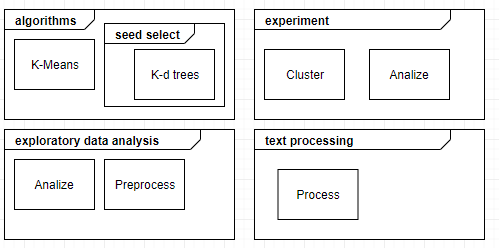
\includegraphics[width=\linewidth]{resources/design.png}
		\caption{Overview of the application packages}
		\label{fig:design}
	\end{figure}
		
	\subsection{Parameters}
	The most important parameter used in the experiment is k, the number of clusters. This was chosen to be the number of distinct beer styles in the dataset, 9, as the reviews for beers of the same type should be similar to each other.
	
	The number of features for each data point is equivalent to how many word frequencies are considered. This was determined experimentally by running the basic algorithm with some different feature values. The results, shown in table \ref{tab:features}, indicate that until around 1000 there is the biggest growth in performance.
	
	\begin{center}
		\label{tab:features}
		\begin{tabular}{ |c|c|c|c| } 
			\hline
			Nr features & Precision & Recall & F1 \\
			\hline
			200 & 0.420 & 0.481 & 0.449 \\
			700 & 0.501 & 0.554 & 0.526 \\
			1000 & 0.537 & 0.532 & 0.534 \\
			1500 & 0.515 & 0.528 & 0.521 \\
			\hline
		\end{tabular}
	\end{center}

	Two methods were tested for seed initialization: random points and kd-tree based. The run with kd-trees obtained a 0.47 F1 score while, random initialization got a 0.53 F1 score. This might be caused by finding good starting points through randomness or that the large number of features is not a good fit for the kd-tree data structure.

	\section{Evaluation}
	\subsection{Metrics}
	The direction chosen for evaluation is how well the clusters found separate the initial dataset by beer types. In order to do this, each cluster is labeled with the most common style of beer among its elements. This turns our problem intro a multi-label classification one.
	
	The metrics used are the ones described by Beleites at al.\cite{MultilabelClassification} for multi-class problems. First of all, a confusion matrix is computed, which is a $l\cdot l$ matrix where l is the number of features. Each element (x, y) in the confusion matrix has a value meaning how many times a data point with label x has been classified as having label y. Precision and recall are then calculated for each label, simulating the binary evaluation. 
	
	Precision, also called positive predictive value, is a fraction that represents how many elements classified with a label have been assigned correctly. Recall, also known as sensitivity, is the fraction of instances correctly assigned to a class and all instances from that class. For the binary case, precision and recall can be calculated as in figure \ref{eq:PrecRecall}, where tp, fp, fn stand for true positives, false positives and false negatives. This can be extended to the confusion matrix, for each row, as follows: precision is the fraction of the value on the diagonal and the sum of values on the column, recall is the value on the diagonal divided by the sum of values on the row. The precision and recall of the multi-label classifier can then be computed as the means of the values obtained from the previous step.
	
	\begin{equation}
	\label{eq:PrecRecall}
	precision = \frac{tp}{tp + fp} \quad recall = \frac{tp}{tp + fn}
	\end{equation}
	
	F1 score is a combined measure of precision and recall, used to provide a single measurement for the system. It represents the harmonic mean of the two values, as in figure \ref{eq:F1}, where mp and mr are mean precision and mean recall.
	
	\begin{equation}
	\label{eq:F1}
	F1 = \frac{2 * mp * mr}{mp + mr}
	\end{equation}
	
	\subsection{Results}
	\subsubsection{Multi-label classification score}
	The correlation between the beer styles of the data points and the type that is most prevalent in the resulting clusters was chose as a measure of evaluation. For the best run, the result can be seen in table \ref{tab:results}. These were obtained using the random seed initialization method.
	
	\begin{center}
		\label{tab:results}
		\begin{tabular}{ |c|c| } 
			\hline
			Mean precision & 0.537 \\
			Mean recall & 0.532 \\
			F1 score & 0.534 \\
			\hline
		\end{tabular}
	\end{center}

	\subsubsection{Heatmap}
	In order to better visualize the results a heatmap was generated. Visible in figure \ref{fig:heatmap}, the diagram helps visualize which style of beer is more common in which cluster. As expected, there is a clear separation for most of the dominant styles in each cluster. This is best observed for the following cluster, style pairs: 0 with Porter, 1 with Stout, 2 with Pale Lager, 4 with Wheat Beer, 5 with Belgian Ale, 6 with Fruit/Vegetable Beer and 7 with Barleywine. For cluster 3 there are two dominant classes : Pale Ale and Amber, which can be explained by the fact that Amber is a particular style of ale. For cluster 8 there is no clear majority, meaning it might be a collection of outliers from other styles.
	
	\begin{figure}
		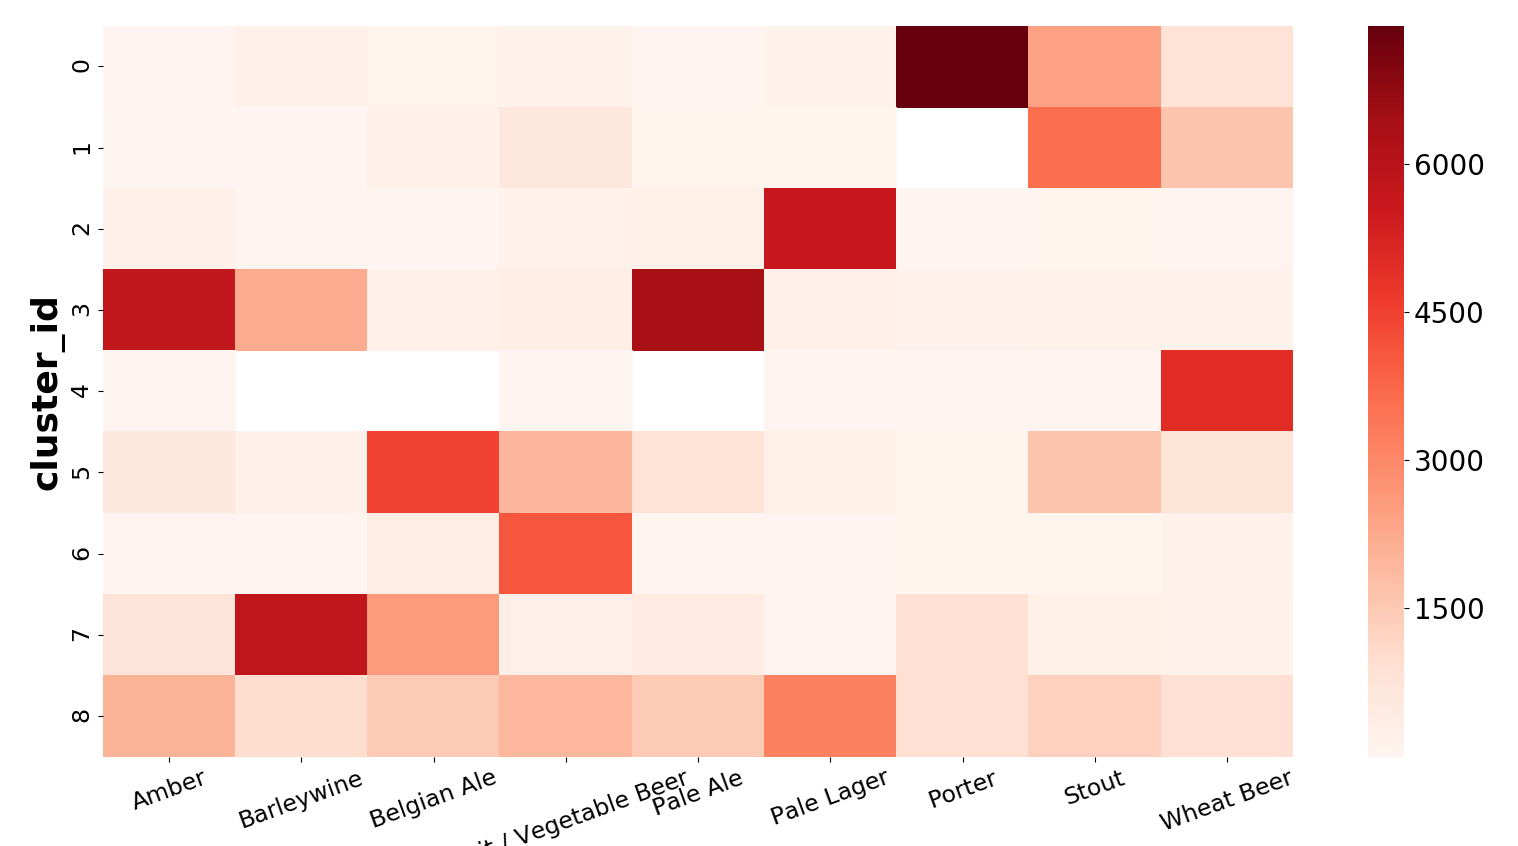
\includegraphics[width=\linewidth]{resources/9500rheatmap.png}
		\caption{Heatmap of beer styles per cluster}
		\label{fig:heatmap}
	\end{figure}
	
	\subsubsection{Common words per cluster}
	In order to interpret what features these clusters have in common, we can look at the most popular words for each cluster, identified by id. Figure \ref{fig:words} shows the 10 words with the highest tf-idf score for the mean of each cluster. Looking at this figure we can find the reason for the shape of cluster 8, as the most common words are general words used in beer description, like 'beer', 'taste', 'drink', 'flavour', which can be applied to any beer style. 
	
	Another thing we can observe from the table of common words is the difference between 'Porter' and 'Stout' styles, which are often put under the same category. According to the diagram, Porter beers tend to have a stronger chocolate, roast, coffee taste while Stouts also have a fruity, citrus taste.
	
	An interesting observation is that while the Wheat Beer style is clearly associated with cluster number 4, the feature words for this cluster: 'chocolate', 'dark', 'roast' are not at all representative of the style.
	
	\begin{figure}
		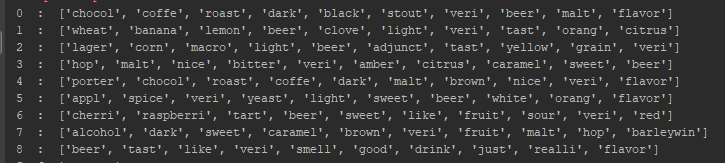
\includegraphics[width=\linewidth]{resources/words.png}
		\caption{Most common words for each cluster}
		\label{fig:words}
	\end{figure}
	
	\section{Conclusions}
	The results of the clustering algorithm were, as expected, clusters around similar beer styles. In terms of multi-label classification the algorithm obtained a F1 score of 0.53 on 9 classes, which indicates there is a correlation. This was also confirmed by the heatmap of the clusters which indicated the poor performance on some of the beer styles. The means of the clusters tend to contain words descriptive of their associated styles with some exceptions.
	
	In terms of improvement, the paper shows that a more sophisticated seed selection method does not offer better results. Another direction worth researching is using more data. This experiment used only 85500 reviews out of the total 1.5 million, which could also be augment with data from other beer review websites. For this to be feasible some computation time optimizations would be useful. 
	
	\newpage
	\bibliography{references_document}
	\bibliographystyle{ieeetr}
\end{document}